\documentclass[10pt]{article}

\usepackage[margin=0.75in]{geometry}
\usepackage{amsmath,amsthm,amssymb}
\usepackage{xcolor}
\usepackage{cancel}
\usepackage{graphicx}
\usepackage{changepage}
\usepackage{circuitikz}
\usepackage{pgfplots}
\usepackage{physics}
\usepackage{hyperref}
\usepackage{siunitx}
\usepackage{multicol, multirow, booktabs}
\usepackage[breakable]{tcolorbox}
\usepackage[inline]{enumitem}

\theoremstyle{definition}
\newtheorem{problem}{Problem}
\newtheorem{soln}{Solution}

\pgfplotsset{compat=newest}
\usetikzlibrary{lindenmayersystems}
\usetikzlibrary{arrows}
\usetikzlibrary{calc}

\definecolor{incolor}{HTML}{303F9F}
\definecolor{outcolor}{HTML}{D84315}
\definecolor{cellborder}{HTML}{CFCFCF}
\definecolor{cellbackground}{HTML}{F7F7F7}
\newcommand{\eq}{=}
\usetikzlibrary{positioning, fit, calc}
\pgfdeclarelayer{background}  
\pgfsetlayers{background,main}
\AtBeginDocument{\RenewCommandCopy\qty\SI}

\makeatletter
\newcommand{\boxspacing}{\kern\kvtcb@left@rule\kern\kvtcb@boxsep}
\makeatother
\newcommand{\prompt}[4]{
    \ttfamily\llap{{\color{#2}[#3]:\hspace{3pt}#4}}\vspace{-\baselineskip}
}

\newcommand{\thevenin}[2]{
  \begin{center}
    \begin{circuitikz} \draw
      (0,0) -- (2,0) to[battery1, l_=$V_{Th}\eq#1$] (2,2) 
      to[resistor, l_=$R_{Th}\eq#2$] (0,2)
      ;
      \draw [o-] (-.07,2.079);
      \draw [o-] (-.07,0.079);
    \end{circuitikz}
  \end{center}
}

\newcommand{\norton}[2]{
  \begin{center}
    \begin{circuitikz} \draw
      (0,0) -- (3,0) to[american current source, l_=$I_{N}\eq#1$] (3,2) -- (0,2) (2,0)
      to[resistor, l=$R_{N}\eq#2$] (2,2)
      ;
      \draw [o-] (-.07,2.079);
      \draw [o-] (-.07,0.079);
    \end{circuitikz}
  \end{center}
}

\newcommand{\highlight}[1]{\colorbox{yellow}{$\displaystyle #1$}}

\newcommand{\ti}[1]{\widetilde{#1}}

\title{Physics 2610H: Assignment IV}
\author{Jeremy Favro}
\date{\today}

\begin{document}
\maketitle

% PROBLEM 1
\begin{problem}
Use the tables of $R(r)$, $\Theta(\theta)$, and $\Phi(\phi)$ to describe the mathematical dependence on the $r$, $\theta$, and $\phi$
variables of the $n = 3$, $\ell=2$, $m_\ell=2$ energy eigenstate of the hydrogen atom. Use computer software of
your choice (Excel, Matlab, \emph{etc.}) to plot the shape of the radial probability density, $P(r)$, of this state
against $r$. Include units! Denote on your plot the most probable radius for an electron in this state.
\end{problem}
\begin{soln} For the $n = 3$, $\ell=2$, $m_\ell=2$ state of the hydrogen atom the wavefunctions are
  $$R(r)=\frac{1}{\left(3a_0\right)^{3/2}}\frac{2\sqrt{2}r^2}{27\sqrt{5}a_0^2}e^{-r/3a_0}$$
  $$\Theta(\theta)=\sqrt{\frac{15}{32\pi}}\sin^2\theta$$
  $$\Phi(\phi)=e^{2i\phi}$$
  The radial wavefunction decays exponentially as we would expect it should. The $\Theta$ component of the angular wavefunction ramps up smoothly to 1
  as the $\theta$ value approaches $\pi/2$. The $\Phi$ component of the angular wavefunction provides an oscillation that is seen more strongly in
  higher quantum numbers and only has one real oscillation before it is killed off by the real valued exponential in the radial component.
  \begin{center}
    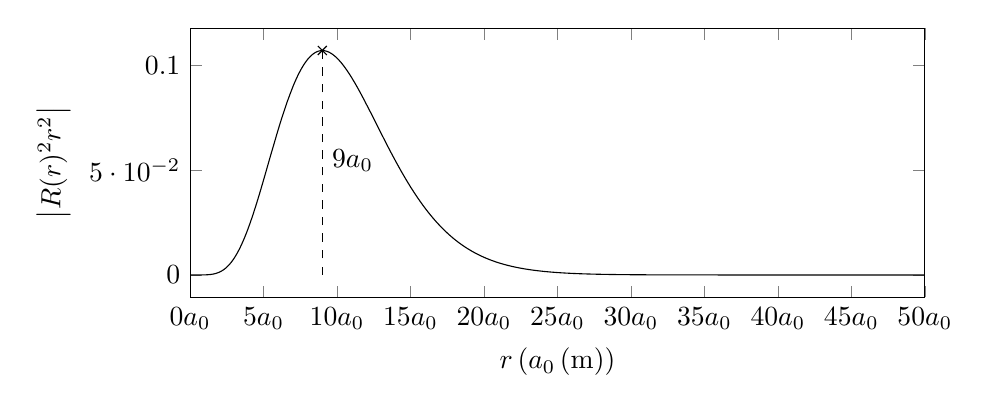
\begin{tikzpicture}
      %\def\a_0{5.292*10^(-11)} This yields the wrong graph for some reason
      \def\a_0{1}
      \begin{axis}[
          width=\textwidth*0.9, height = 5cm,
          xlabel={$r\,(a_0\,(\unit{\meter}))$}, ylabel={$\left|R(r)^2r^2\right|$},
          xticklabel={\pgfmathparse{\tick}${\pgfmathprintnumber{\pgfmathresult}}a_0$},
          xmin=0, xmax=50
        ]
        \addplot[domain=0:50*\a_0, smooth, samples=501]
        (\x,{(((3*\a_0)^(-3/2))*((2*sqrt(2)*\x^2)/(27*sqrt(5)*\a_0^2))*(e^(-\x/(3*\a_0))))^2*\x^2});
        \draw [dashed, -Rays] (9*\a_0,0) -- (9*\a_0,0.1095) node[midway, right]{$9a_0$};
      \end{axis}
    \end{tikzpicture}
  \end{center}
\end{soln}
\newpage

% PROBLEM 2
\begin{problem}
Show that the degeneracy of the $n$-th state of the hydrogen atom \emph{if} the electron had no spin (so course
material only up to Chapter 7) would be $n^2$. That is, prove the following equality and in a sentence or two
state why this equation answers this question:
$$\sum_{\ell=0}^{n-1}\left(2\ell+1\right)=n^2$$
\end{problem}
\begin{soln}
  Note the sum is
  $$\sum_{\ell=0}^{n-1}(2\ell+1)=1+(2+1)+\dots+(2(n-1)+1)$$
  which is the sum of odd integers up to $n-1$. The sum we are interested in can be split into two parts,
  $$\sum_{\ell=0}^{n-1}(2\ell)+\sum_{\ell=0}^{n-1}1$$
  The second part of this sum, $\sum_{\ell=0}^{n-1}1$, is the sum of $1$ $n-1+1$ times, the $+1$ arising due to the beginning index being at
  $0$ (Fencepost problem! That took me a minute). This reduces to $n$.
  $\sum_{\ell=0}^{n-1}(2\ell)$ is simply twice the sum of the integers up to $n-1$ which is equal to
  $$(n-1)(n)$$
  so the entire sum is
  $$(n-1)(n)+(n)=n^2.$$
  This equation gives the degeneracy of the $n$-th state of the hydrogen atom as $\ell$ runs from $0$ to $n-1$ and $m_\ell$ runs from $-\ell$ to $+\ell$
  which means $m_\ell$ could be any value from $0$ to $\pm(n-1)$. Because degeneracy (without spin) is effectively a
  measure of the number of possible values of $m_\ell$ the degeneracy can be expressed as the sum given in the problem statement.
\end{soln}
\newpage

% PROBLEM 3
\begin{problem}
For a hydrogen atom in the $1s$ state
\begin{enumerate}[label=(\alph*)]
  \item What is the most probable value of $r$ from a measurement of $r$?
  \item What is the average value of $r$?
  \item Where in 3-dimensional space is the electron most likely to be within a small volume of \underline{fixed} size $dV$?
\end{enumerate}
\end{problem}
\begin{soln}~
  \begin{enumerate}[label=(\alph*)]
    \item Here we are looking for the maximum of the probability,
          $$R^2(r)r^2=\left(\frac{2e^{-r/a_0}}{a_0^{3/2}}\right)^2r^2=\frac{4r^2e^{-2r/a_0}}{a_0^3}=P(r)$$
          This can be found by solving
          $$\frac{dP}{dr}=\frac{8r(r-a_0)e^{-2r/a_0}}{a_0^4}=0$$
          Which gives solutions of $r=0,a_0,\infty$. $0$ and $\infty$ are non-physical so the most probable value is $r=a_0$.
    \item $$\int_0^\infty R^2(r)r^3\,dr
            =\int_0^\infty\left(\frac{2e^{-r/a_0}}{a_0^{3/2}}\right)^2r^3\,dr
            =\frac{4}{a_0^{3}}\int_0^\infty r^3e^{-2r/a_0}\,dr$$
          Which, using the integral table given on the formula sheet, is
          $$\frac{4}{a_0^{3}}\frac{3!}{\left(\frac{2}{a_0}\right)^4}=\frac{3a_0}{2}$$
    \item The probability density is maximum at the origin. Though this is nonphysical and does not align with the answer in (a) it makes sense
          when looking at a probability density plot of the $1s$ state. The inconsistency between this and part (a) can be resolved by noting that
          the radial probability considers a sphere of thickness $dr$ centered about the origin with greatest probability density being where this sphere
          ``intersects'' the greatest ``amount of probability'' whereas the probability of a fixed volume is measured with a region of infinitesimal
          volume $dV$. Noting this the apparent inconsistency disappears as they are fundamentally different measurements.
  \end{enumerate}
\end{soln}

% PROBLEM 4
\begin{problem}
Evaluate, in electron volts, the energies of the three lowest energy levels of the hydrogen atom. Then
calculate the frequencies in $\unit{\hertz}$, and the wavelengths in $\unit{\angstrom}$ of all the photons that can be emitted by the
atom in transitions between these levels. In what range of the electromagnetic spectrum are these photons?
\end{problem}
\begin{soln}
  The energy levels of the hydrogen atom can be expressed as a function of the principle quantum number, $n$, only. These
  energies are given by the equation
  $$E(n)=-\frac{mZ^2e^4}{\left(4\pi\epsilon_0\right)2\hbar^2n^2}\approx-\frac{\qty{13.6}{\electronvolt}}{n^2}$$
  which gives energy levels of $\qty{-13.6}{\electronvolt}$, $\qty{-3.4}{\electronvolt}$, and $\qty{-1.51}{\electronvolt}$
  for $n=1,2,3$. For frequencies associated with these transitions we only have to care about downward movement so we have
  \begin{align*}
    3\to 2  : & \lambda=\frac{hc}{\Delta E}\approx\frac{hc}{\qty{-3.4}{\electronvolt}-\qty{-13.6}{\electronvolt}}\approx\qty{1.22}{\kilo\angstrom}
    \implies f\approx\qty{2.47d15}{\hertz}                                                                                                         \\
    3\to 1  : & \approx\qty{1.02}{\kilo\angstrom}\implies f\approx\qty{2.92d15}{\hertz}                                                            \\
    2\to 1  : & \approx\qty{6.56}{\kilo\angstrom}\implies f\approx\qty{4.57d14}{\hertz}
  \end{align*}
  The the first two transitions emit photons in the ultraviolet range and the last emits a photon in the near infrared range.
\end{soln}
\newpage

% PROBLEM 5
\begin{problem}
Consider the probability of finding the electron in the hydrogen atom somewhere inside a cone of $\theta=\qty{23.5}{\degree}$
(``arctic polar region'').
\begin{enumerate}[label=(\alph*)]
  \item If the electron were equally likely to be found anywhere in space, what would be the probability of finding the
        electron in the arctic polar region?
  \item Suppose the electron is in the state $n = 2$, $\ell = 1$, $m_\ell = 0$ (i.e. a $2p_z$ orbital); recalculate the probability of
        finding the electron in the arctic polar region.
\end{enumerate}
\end{problem}
\begin{soln}~
  \begin{enumerate}[label=(\alph*)]
    \item Because the probability distribution here is uniform we are looking for how much volume the arctic polar region occupies out of the total sphere.
          This is somewhat difficult to determine as both are technically infinite but by evaluating the improper integral we get using a limit the final answer is finite.
          \begin{align*}
            = & \lim_{R\to\infty}\frac{1}{\frac{4}{3}\pi r^3}\int_{0}^{47\pi/360}\int_{0}^{2\pi}\int_0^R r^2\sin\theta\,dr d\phi d\theta \\
            = & -\lim_{R\to\infty}\frac{1}{\frac{4}{3}\pi r^3}\eval{\frac{2\pi r^3\cos\theta}{3}}_{r=0,\theta=0}^{r=R,\theta=47\pi/360}  \\
            = & -\eval{\frac{\cos\theta}{2}}_{\theta=0}^{\theta=47\pi/360}\approx 4.15\%
          \end{align*}
    \item \begin{align*}
            = & \iiint \left(\frac{1}{\left(2a_0\right)^{3/2}}\frac{r}{\sqrt{3}a_0}e^{-r/2a_0}\sqrt{\frac{3}{4\pi}}\cos\theta\right)^2r^2\sin\theta\,dV \\
            = & \frac{1}{16a_0^5}\iint r^4e^{-r/a_0}\cos^2\theta\sin\theta\,dr d\theta                                                                  \\
            = & \frac{3}{2}\int \cos^2\theta\sin\theta\,d\theta                                                                                         \\
            = & \eval{-\frac{\cos^3(\theta)}{2}}_{0}^{47\pi/360}\approx 11.4\%
          \end{align*}
  \end{enumerate}
\end{soln}

% PROBLEM 6
\begin{problem}
An electron (with spin) in a hydrogen atom is in the $4f_{5/2}$ state. Find the values of the quantum numbers
$n$, $\ell$ and $j$. What is the magnitude of the electron's total angular momentum? What are the possible values
for the $z$-component of the electron's total angular momentum?
\end{problem}
\begin{soln}
  $n=4$, $\ell=3$, $j=\left|\ell-s\right|=\left|3-\frac{1}{2}\right|=5/2$.
  $\| \vec{J}\Vert =\| \vec{L}+ \vec{S}\Vert=\left(\sqrt{\ell(\ell+1)}+\sqrt{s(s+1)}\right)\hbar=\frac{5\sqrt{3}}{2}\hbar$.
  $J_z=m_j\hbar=\left\{-j,-j+1,\dots, j-1, j\right\}\hbar=\left\{-5/2,-3/2,-1/2, 1/2, 3/2, 5/2\right\}\hbar$.
\end{soln}
\newpage

% PROBLEM 7
\begin{problem}
Neglecting any effects of spin (i.e. if both particles are spinless), how many quantum states are possible
for a two-particle system with orbital angular momentum quantum numbers $\ell_1=2$ and $\ell_2=1$? Write down
all these states in what is called the \emph{uncoupled} form: ($\ell_1m_{\ell_1}\ell_2m_{\ell_2}$). Then find all possible values of the
total orbital angular momentum quantum number $\ell_T$ and the total orbital magnetic quantum number $m_{\ell_T}$. Write down all these states
in the \emph{coupled} form: ($\ell_1\ell_2\ell_Tm_{\ell_T}$).
\end{problem}
\begin{soln} For such a system there are 15 possible states. This arises because there are five values of $m_{\ell_1}$ ($-2,-1,0,1,2$) and
  three of $m_{\ell_2}$ ($-1,0,1$) and $5\cdot 3 = 15$. Each possible combination in both forms is tabulated below,
  \begin{table}[h!]
    \centering%
    \begin{tabular}{l}
      \toprule
      Uncoupled      \\
      \midrule
      ($2(-2)1(-1)$) \\
      ($2(-2)10$)    \\
      ($2(-2)11$)    \\
      ($2(-1)1(-1)$) \\
      ($2(-1)10$)    \\
      ($2(-1)11$)    \\
      ($201(-1)$)    \\
      ($2010$)       \\
      ($2011$)       \\
      ($211(-1)$)    \\
      ($2110$)       \\
      ($2111$)       \\
      ($221(-1)$)    \\
      ($2210$)       \\
      ($2211$)       \\
      \bottomrule
    \end{tabular}\qquad
    \begin{tabular}{l}
      \toprule
      Coupled       \\
      \midrule
      ($21 1 (-1)$) \\
      ($21 1 (0)$)  \\
      ($21 1 (1)$)  \\
      ($21 2 (-2)$) \\
      ($21 2 (-1)$) \\
      ($21 2 0$)    \\
      ($21 2 1$)    \\
      ($21 2 2$)    \\
      ($21 3 (-3)$) \\
      ($21 3 (-2)$) \\
      ($21 3 (-1)$) \\
      ($21 3 0$)    \\
      ($21 3 1$)    \\
      ($21 3 2$)    \\
      ($21 3 3$)    \\
      \bottomrule
    \end{tabular}
  \end{table}
\end{soln}

% PROBLEM 8
\begin{problem}
Two spinless particles, assumed initially to be distinguishable from each other, occupy two different
states ($n=2$ and $n^\prime=3$) in a 1-D infinite well of length $L$. The \emph{product wave function} for the case with particle 1 in
state $n=2$ and particle 2 in state $n^\prime=3$ is
$$\psi(x_1,x_2)=A\sin\left(\frac{2\pi x_1}{L}\right)\sin\left(\frac{3\pi x_2}{L}\right),\qquad A=\frac{2}{L}$$
\begin{enumerate}[label=(\alph*)]
  \item Show that with this normalization constant this product wave function is correctly normalized.
  \item If the two particles are instead \emph{identical} how should this product wave function be adapted to form two
        realistic wave functions? Given that the normalization constant for each of these wave functions is $L=\sqrt{2}/L$
        in each case what is the probability of both particles being found in the left half of the well (i.e. between $0$ and $L/2$).
\end{enumerate}
\end{problem}
\begin{soln}~
  \begin{enumerate}[label=(\alph*)]
    \item \begin{align*}
            = & \int_{0}^{L}\int_{0}^{L}A^2\sin^2\left(\frac{2\pi x_1}{L}\right)\sin^2\left(\frac{3\pi x_2}{L}\right)\,dx_1dx_2                                                                             \\
            = & \frac{A^2}{4}\int_{0}^{L}\int_{0}^{L}\left(1-\cos\left(\frac{4\pi}{L}x_1\right)\right)\left(1-\cos\left(\frac{6\pi}{L}x_2\right)\right)\,dx_1dx_2                                           \\
            = & \frac{A^2}{4}\int_{0}^{L}\int_{0}^{L}1-\cos\left(\frac{4\pi}{L}x_1\right)-\cos\left(\frac{6\pi}{L}x_2\right)+\cos\left(\frac{4\pi}{L}x_1\right)\cos\left(\frac{6\pi}{L}x_2\right)\,dx_1dx_2 \\
            = & \frac{A^2}{4}\int_{0}^{L}\left[x_1x_2-\frac{Lx_2}{4\pi}\sin\left(\frac{4\pi}{L}x_1\right)
              -\frac{Lx_1}{6\pi}\sin\left(\frac{6\pi}{L}x_2\right)
              + \frac{L^2}{24\pi^2}\sin\left(\frac{4\pi}{L}x_1\right)\sin\left(\frac{6\pi}{L}x_2\right)
            \right]_0^L                                                                                                                                                                                     \\
            = & \frac{A^2}{4}\int_{0}^{L}\left[x_1x_2-\frac{Lx_2}{4\pi}\sin\left(\frac{4\pi}{L}x_1\right)
              -\frac{Lx_1}{6\pi}\sin\left(\frac{6\pi}{L}x_2\right)
              + \frac{L^2}{24\pi^2}\sin\left(\frac{4\pi}{L}x_1\right)\sin\left(\frac{6\pi}{L}x_2\right)
            \right]_0^L                                                                                                                                                                                     \\
            = & \frac{A^2}{4}\cdot L^2=\frac{4}{4L^2}\cdot L^2=1
          \end{align*}
    \item Dependent on whether the particles are fermions or bosons the wavefunction must be made antisymmetric or symmetric,
          e.g. $\psi(x_1,x_2)=-\psi(x_2,x_1)$ for fermions (antisymmetric) and $\psi(x_1,x_2)=\psi(x_2,x_1)$ for bosons (symmetric).
          This can be accomplished by either adding or subtracting a copy of the given wavefunction with flipped particle identifiers,
          \begin{align*}
             & \sin\left(\frac{2\pi x_1}{L}\right)\sin\left(\frac{3\pi x_2}{L}\right)-\sin\left(\frac{2\pi x_2}{L}\right)\sin\left(\frac{3\pi x_1}{L}\right)\qquad\text{Antisymmetric} \\
             & \sin\left(\frac{2\pi x_1}{L}\right)\sin\left(\frac{3\pi x_2}{L}\right)+\sin\left(\frac{2\pi x_2}{L}\right)\sin\left(\frac{3\pi x_1}{L}\right)\qquad\text{Symmetric}
          \end{align*}
          As for probability we need to evaluate the integrals
          $$\frac{2}{L^2}\int_{0}^{L/2}\int_{0}^{L/2}\left(\sin\left(\frac{2\pi x_1}{L}\right)\sin\left(\frac{3\pi x_2}{L}\right)-\sin\left(\frac{2\pi x_2}{L}\right)\sin\left(\frac{3\pi x_1}{L}\right)\right)^2\,dx_1dx_2$$
          $$\frac{2}{L^2}\int_{0}^{L/2}\int_{0}^{L/2}\left(\sin\left(\frac{2\pi x_1}{L}\right)\sin\left(\frac{3\pi x_2}{L}\right)+\sin\left(\frac{2\pi x_2}{L}\right)\sin\left(\frac{3\pi x_1}{L}\right)\right)^2\,dx_1dx_2$$
          For the antisymmetric integral,
          \begin{align*}
             & = \frac{2}{L^2}\int_{0}^{L/2}\int_{0}^{L/2}\left(\sin\left(\frac{2\pi x_1}{L}\right)\sin\left(\frac{3\pi x_2}{L}\right)-\sin\left(\frac{2\pi x_2}{L}\right)\sin\left(\frac{3\pi x_1}{L}\right)\right)^2\,dx_1dx_2                                                    \\
             & = \frac{2}{L^2}\int_{0}^{L/2}\int_{0}^{L/2}\sin^2\left(\frac{2\pi x_1}{L}\right)\sin^2\left(\frac{3\pi x_2}{L}\right)-2\sin\left(\frac{2\pi x_1}{L}\right)\sin\left(\frac{3\pi x_2}{L}\right)\sin\left(\frac{2\pi x_2}{L}\right)\sin\left(\frac{3\pi x_1}{L}\right)+ \\
             & \qquad \sin^2\left(\frac{2\pi x_2}{L}\right)\sin^2\left(\frac{3\pi x_1}{L}\right)\,dx_1dx_2                                                                                                                                                                          \\
             & = \frac{2}{L^2}\left[\frac{L^2}{16}-\frac{L^2}{2\pi^2}\left(1-\frac{1}{5}\right)^2+\frac{L^2}{16}\right] \quad \text{(Integral formulas borrowed from the text.)}                                                                                                    \\
             & \approx 4.63\%
          \end{align*}
          For the symmetric integral we repeat the same process but flip the sign when expanding the binomial so we end up with
          $$\frac{2}{L^2}\left[\frac{L^2}{16}+\frac{L^2}{2\pi^2}\left(1-\frac{1}{5}\right)^2+\frac{L^2}{16}\right]\approx45.4\%$$
  \end{enumerate}
\end{soln}
\end{document}